\documentclass[12pt]{article}
\usepackage[utf8]{inputenc}
\usepackage[T1]{fontenc}
\usepackage{xspace}
\usepackage[french]{babel}
\usepackage{geometry}
\usepackage{graphicx}
\usepackage{float}
\usepackage{caption}
\usepackage{array}
\usepackage{lscape}
\usepackage{listings}
\usepackage[dvipsnames]{xcolor}
\usepackage[hidelinks]{hyperref}

\geometry{hmargin=2.5cm,vmargin=2.5cm}
\lstset{
	language=C,
	backgroundcolor=\color{black!5!white},
	basicstyle=\normalsize,
	commentstyle=\color{OliveGreen},
	keywordstyle=\color{blue},
	morekeywords={uint32_t},
	frame=single,
	numbers=left,
	tabsize=3
}

\title{Rapport Realtime Oscilloscope}
\author{Martin Meyer}
\date{06 Mai 2020}

\begin{document}

	\maketitle
	
	\tableofcontents

	\section{Introduction}
	Dans ce laboratoire, nous avons créé un système temps réel réalisant un fonction d'oscilloscope. Une partie des tâches, comme l'échantillonnage, fonctionne en temps réel. D'autre tâches, comme l'affichage, n'en ont pas besoin.\\
	Pour ce faire, nous avons travaillé avec les cartes microcontrôleur STM32f7-discovery, System Workbench for STM32 et STM32CubeMX.\\
	Ce rapport décrit quelques parties intéressantes du programme, notamment grâce à des diagrammes UML.\newpage
	\section{Diagrammes}
	\subsection{Diagramme de timing}
	Ci-dessous, le diagramme de timing:
	\begin{figure}[H]
		\begin{center}
			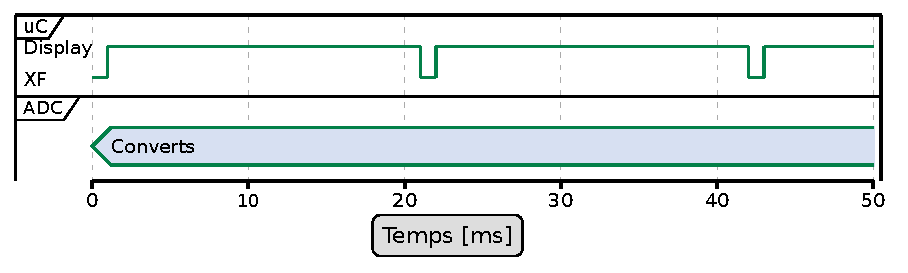
\includegraphics[width=\columnwidth]{Ressources/timing.pdf}
			\caption{\label{timing} Diagramme de timing}
		\end{center}
	\end{figure}
	On peut voir sur la figure \ref{timing} que l'affichage prend environ 20ms. Il s'en suit un court passage dans le XF. L'adc est considéré comme toujours actif, car il fait une conversion toutes les 10 us.
	\subsection{Diagramme de classe}
	\begin{figure}[H]
	\begin{center}
		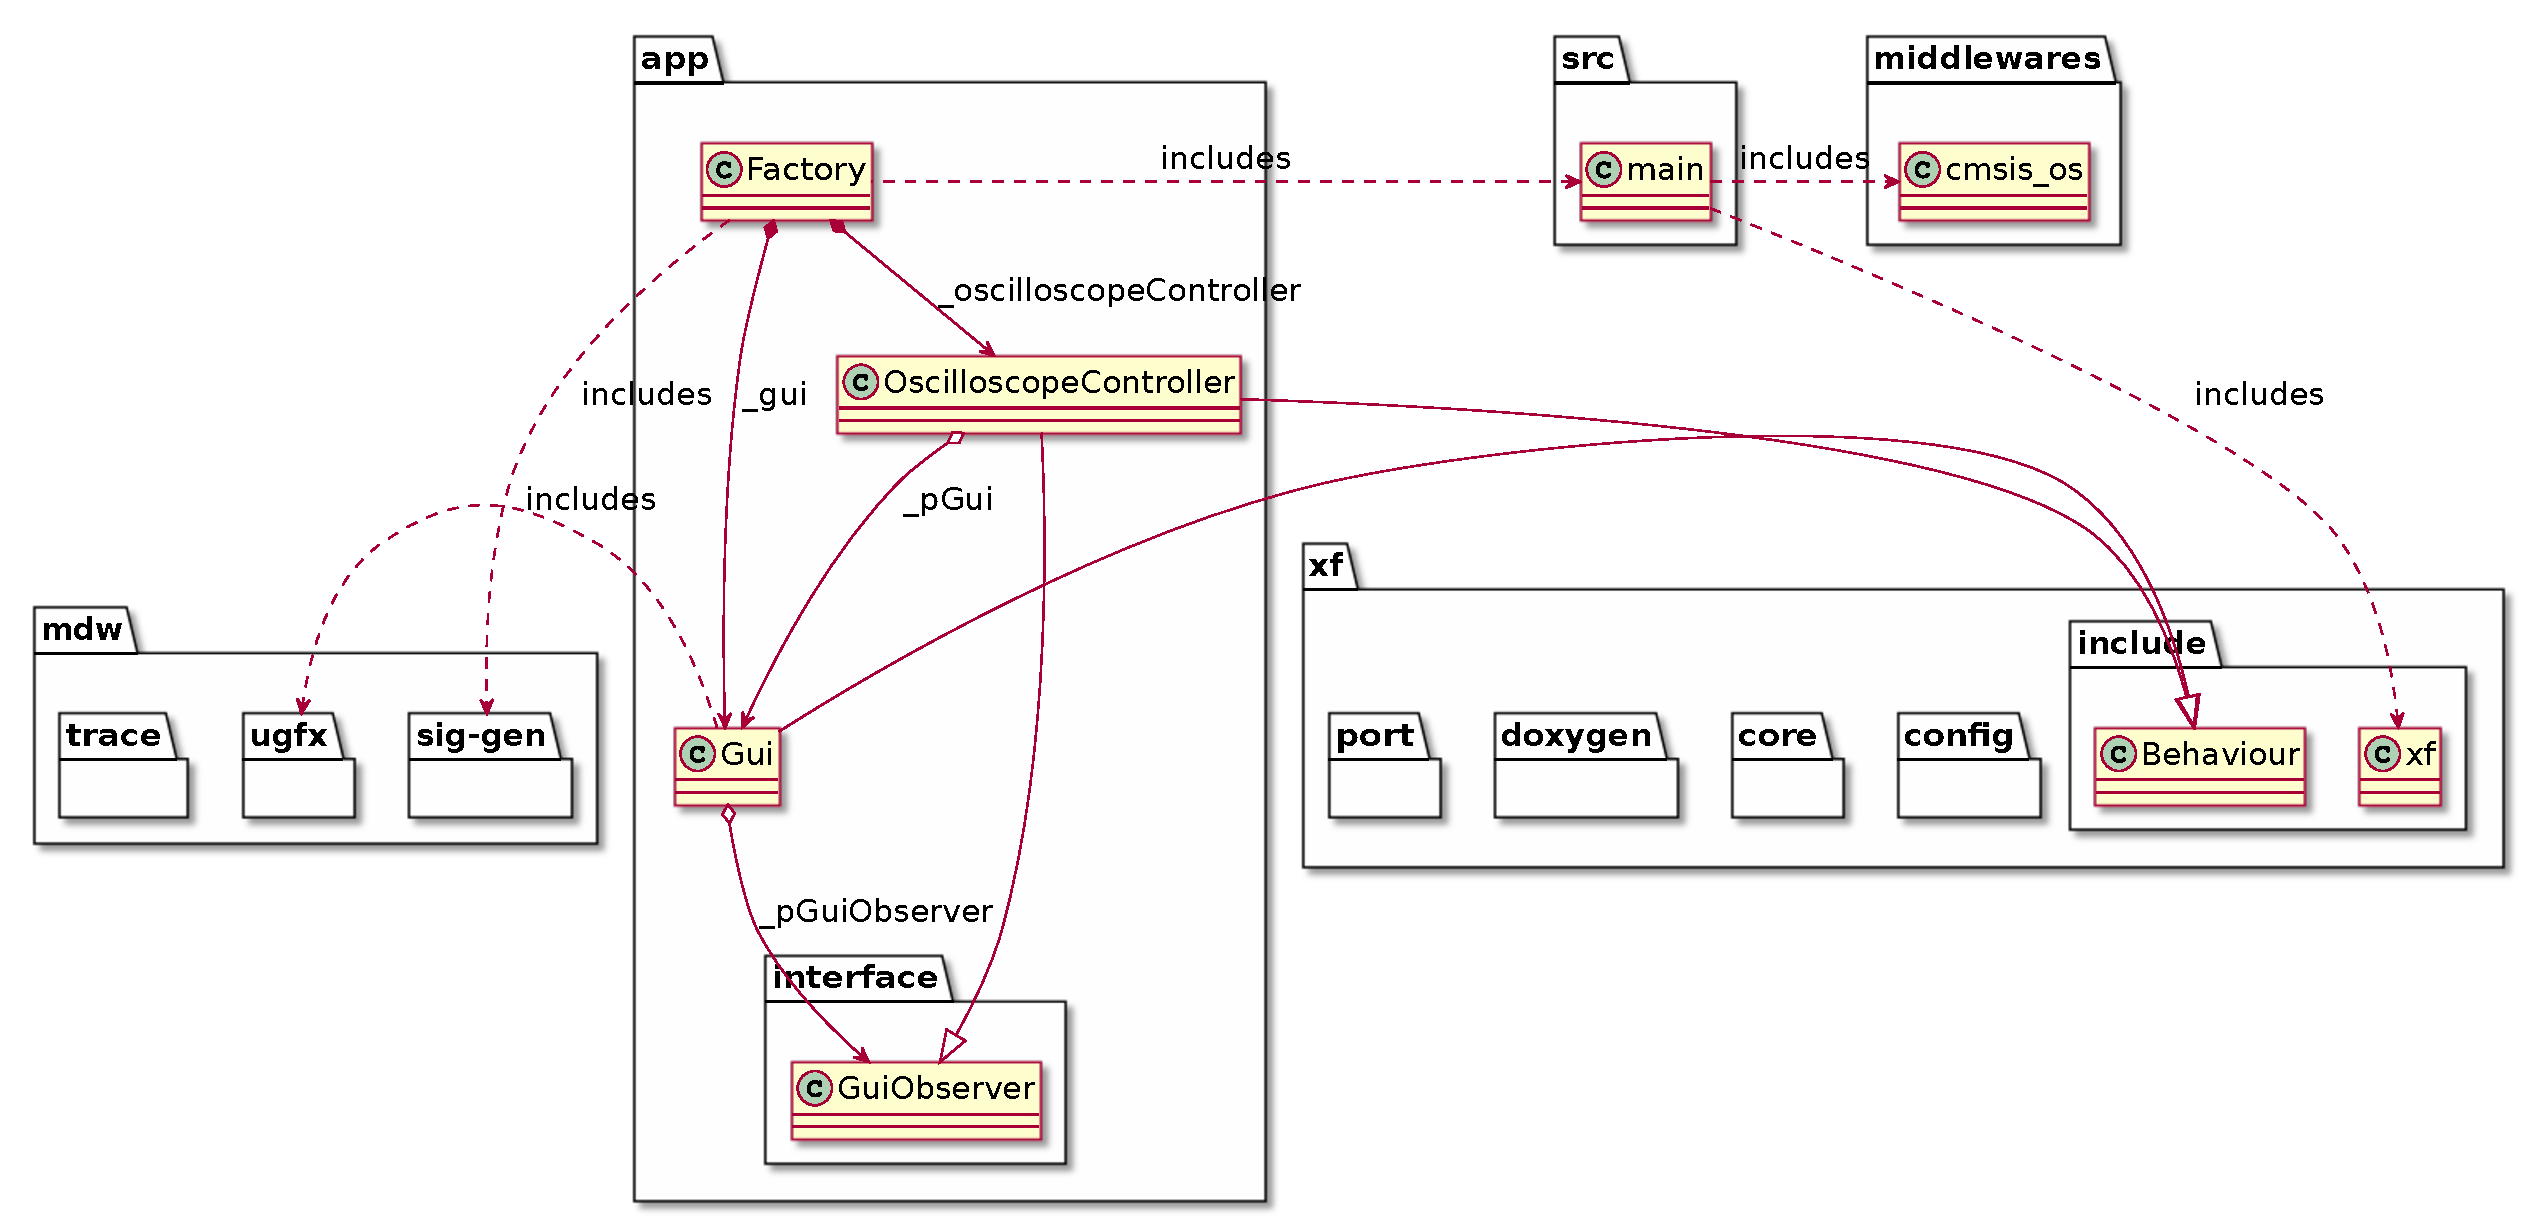
\includegraphics[angle=270,scale=0.45]{Ressources/class.pdf}
		\caption{\label{class} Diagramme de classe}
	\end{center}
\end{figure}
	\section{Patterns}
	\subsection{Singleton}
	Le pattern singleton est utilisé dans plusieurs classes, commme la Factory ou l'OscilloscopeController.
	\subsection{Sujet-observateur}
	Un pattern sujet-observateur est utilisé. La classe OscilloscopeController est l'observateur et la classe Gui le sujet.
	\subsection{Factory}
	Une Factory est utilisée dans ce labo. Elle initialise des relations et lance le système.
	\section{Questions}
	\subsection{Tâche 6}
	\subsubsection{Question 1}
	\textbf{Est-ce qu'il est possible d'exécuter le composant numéro 1 avec un XF ou bien faut-il un RTOS ? Justifiez votre réponse.}\\
	Non, étant donné le timing de conversion du signal analogique qui est court, le processeur passerait trop de temps dans les switching context ou dans le xf. Il est préférable d'utiliser une timer hardware dans ce cas.
	\subsubsection{Question 2}
	\textbf{Est-ce qu'il est possible d'exécuter le composant numéro 2 avec un XF ou bien faut-il un RTOS ? Justifiez votre réponse.}\\
	Oui, c'est possible, car le taux de rafraichissement est suffisament bas pour utiliser un XF ou un RTOS.
	\subsubsection{Question 3}
	\textbf{Si l'on combine un timer hardware avec un XF, lequel des deux doit être priorisé ? Justifiez votre réponse.}\\
	Il faut prioriser le timer hardware, car il est plus important d'avoir un échantillonnage précis plutôt qu'un affichage précis. De plus, comme un rafraîchissement de l'écran dure plusieurs milliseconds, la conversion du signal analogique serait bloquée pendant ce temps.	
	\subsection{Tâche 8}
	\subsubsection{Question 1}
	\textbf{Combien de mesures [Samples/s] le convertisseur A/D doit-il effectuer par seconde pour pouvoir échantillonner des signaux avec des fréquences jusqu'à 1 kHz ?}\\
	Le théorème de Shannon nous dit que la fréquence d'échantillonnage doit être au moins 2 fois plus grande que la fréquence du signal à échantilloné. On devrait donc faire au moins 2kSamples/s. Cependant, pour avoir un signal lisible, il faudrait au moins avoir une fréquence de sampling de 20kSamples/s.
	\subsubsection{Question 2}
	\textbf{Faut-il un filtre ? Si oui, quelle sera la fréquence de coupure de ce filtre ?}\\
	Oui, il faut ajouter un filtre passe-bas à l'entrée du signal à mesurer avec une fréquence de coupure à 1kHz, afin d'éviter que des signaux avec une fréquence plus élevée fausse les mesures, par un phénomène de sous-échantillonnage.
	\subsubsection{Question 3}
	\textbf{Est-ce que la fréquence donnée par le théorème d’échantillonnage ou devrait-elle être plus élévée ?}\\
	La fréquence doit être plus élevée (par exemple 10kSamples/s) pour avoir un signal lisible. Si l'on utilise la fréquence donnée par le théorème d'échantillonnage, on aura seulement 2 points de mesure par période.
	\subsubsection{Question 4}
	\textbf{Lequel des canaux du ADC3 doit être utilisé pour pouvoir mesurer / échantillonner le signal à l'aide de la broche PA0 ?}\\
	Le canal IN0.
	\subsubsection{Question 5}
	\textbf{Est-ce que le ADC pourrait-il éventuellement effectuer des mesures à des intervalles réguliers à l'aide de ses propres moyens ?}\\	
	Oui il le pourrait, en mode continu. Mais on ne pourrait pas choisir l'intervalle de ces conversions, car l'ADC relancerait une nouvelle conversion automatiquement directement après qu'une conversion soit finie.
	\subsection{Tâche 14}
	\subsubsection{Question 1}
	\textbf{Quelle fréquence d’échantillonnage peut être atteinte?}\\
	La fréquence d'échantillonnage maximale atteinte est de 250kSamples/s.
	\subsubsection{Question 2}
	\textbf{Quel(s) composant(s) limite(nt) le système?}\\
	Le temps d'interruption qui limite le système. Lorsque la fréquence d'échantillonnage est trop élevée, le processeur va être tout le temps dans l'interruption de fin de conversion ADC. Le clock et la mémoire limitent le système, car en les augmentant, on pourrait augmenter la fréquence de sampling.
	
	\subsection{Tâche 15}
	\subsubsection{Question 1}
	\textbf{À quelle fréquence maximale peut-on régler l’échantillonnage?}\\
	On peut la régler à 250kSamples/s au maximum.
	\subsubsection{Question 2}
	\textbf{Quels avantages voyez-vous à utiliser FreeRTOS dans cette application?}\\
	Avec des sytèmes qui fonctionnent à des grandes fréquences (plus de 1kHz), un RTOS devient intéressant car il permet d'utiliser des priorités entre différentes tâches. Dans notre cas, le timer serait par exemple priorisé.
	\subsubsection{Question 3}
	\textbf{Donnez un exemple où un RTOS serait particulièrement nécessaire?}\\
	Par exemple un système d'arrêt d'urgence doit être priorisé sur toutes les autres tâches.
	\section{Tâches facultatives}
	\subsection{FA1 - Fonction trigger}
	Le but de cette fonction est d'afficher le signal d'une façon à ce qu'il reste toujours au même endroit sur l'écran et d’éviter qu’il se déplace à travers de l'écran.\\
	Le seuil du trigger a été fixé à 2048 arbitrairement. Cette valeur correspond à la moitié de la plage de valeur de l'ADC. La fonctionnalité trigger est implémentée dans la méthode doShowAnalogSignal() de la classe OscilloscopeController.\\
	
		\begin{figure}[H]
		\begin{lstlisting}
if(TriggerOn){
	uint32_t temp_low=0;
	uint32_t temp_high=0;
	uint32_t nbMoy=5;
	for(int i=nbMoy;i<_adcValuesBufferSize-size-nbMoy;i++){
		for(int j=0;j<nbMoy;j++){//Points average loop
			temp_low+=_adcValuesBuffer[i-j];
			temp_high+=_adcValuesBuffer[i+j];
		}
		temp_low/=nbMoy;
		temp_high/=nbMoy;
	
		//check the trigger value
		if(temp_low<triggerValue&&temp_high>triggerValue){
			//update the pointer
			trigPtr = &_adcValuesBuffer[i];
		}
	}
}
else{
	trigPtr = _adcValuesBuffer;
}

gui().drawGraphPoints(trigPtr, size,xScale);
		\end{lstlisting}
		\caption{Trigger Code}
		\label{code_trig}
	\end{figure}
La figure \ref{code_trig} montre le code du trigger. On va rechercher l'index du tableau de mesures auquel le niveau des mesures devient plus élevé que le seuil du trigger. Pour plus de précision, une moyenne de 5 points est effectuée. Une fois que le seuil est détecté, le pointer passé à la fonction drawGraphPoint est mis à jour.	
	\subsection{FA2 - Axe du temps}
	Pour calculer le paramètre xScale de la méthode drawPoints, l'équation suivante a été utilisée:
	\begin{equation}
	\frac{600}{tDiv\cdot\frac{8}{tSample}}
	\end{equation}
	Le 600 correspond au nombre de pixel en x à afficher, et le 8 est le nombre de division.
	Elle a ensuite été transformée pour ne pas utiliser des float avec une valeur trop petite:
	\begin{equation}
		\frac{600}{fSample\cdot\frac{8}{fDiv}}
	\end{equation}
	Malgré ce calcul, l'échelle n'était pas correct. J'ai donc ajouté un facteur pour que tout fonctionne. L'équation finale:
	\begin{equation}
	\frac{600}{fSample\cdot\frac{8}{fDiv}}\cdot 1.7
	\end{equation}
	\section{Tests}
	\subsection{A}
		\begin{table}[H]
			\begin{center}
				\begin{tabular}{| m{2cm}|m{2cm}|m{12cm}|}
					\hline 
					\bf A1&\bf Title:&\bf Check if ADC Signal acquisition is working\\ 
					\hline 
					\multicolumn{2}{|c|}{Group:}&Signal Acquisition\\ 
					\hline 
					\multicolumn{2}{|c|}{Description:}&Is buffer continuously feed with new ADC measures?
					\\ 
					\hline 
					\multicolumn{2}{|c|}{Initial Conditions:}&Running program\\ 
					\hline 
					\multicolumn{2}{|c|}{Test Results:}&The buffer is continuously feed with new ADC measures.\\ 
					\hline 
					\multicolumn{2}{|c|}{Final Conditions:}&Running program\\ 
					\hline 
					\multicolumn{2}{|c|}{Comments:}&\\ 
					\hline 
					\multicolumn{2}{|c|}{Test Passed:}&Yes\\ 
					\hline 
				\end{tabular} 
			\end{center}
		\end{table}
	
		\begin{table}[H]
			\begin{center}
				\begin{tabular}{| m{2cm}|m{2cm}|m{12cm}|}
					\hline 
					\bf A2&\bf Title:&\bf Check TIM1 continously trigger the ADC\\ 
					\hline 
					\multicolumn{2}{|c|}{Group:}&Signal Acquisition\\ 
					\hline 
					\multicolumn{2}{|c|}{Description:}&Not software trigger, nor ADC continous conversion mode\\ 
					\hline 
					\multicolumn{2}{|c|}{Initial Conditions:}&Running program\\ 
					\hline 
					\multicolumn{2}{|c|}{Test Results:}&Yes, the ADC conversion is started directly from the TIM1 timeout signal.\\ 
					\hline 
					\multicolumn{2}{|c|}{Final Conditions:}&Running program\\ 
					\hline 
					\multicolumn{2}{|c|}{Comments:}&\\ 
					\hline 
					\multicolumn{2}{|c|}{Test Passed:}&Yes\\ 
					\hline 
				\end{tabular} 
			\end{center}
		\end{table}	
	
			\begin{table}[H]
		\begin{center}
			\begin{tabular}{| m{2cm}|m{2cm}|m{12cm}|}
				\hline 
				\bf A3&\bf Title:&\bf Check TIM1 trigger frequency\\ 
				\hline 
				\multicolumn{2}{|c|}{Group:}&Signal Acquisition\\ 
				\hline 
				\multicolumn{2}{|c|}{Description:}&Is TIM1 trigger frequency as expected?\\ 
				\hline 
				\multicolumn{2}{|c|}{Initial Conditions:}&-\\ 
				\hline 
				\multicolumn{2}{|c|}{Test Results:}&Test can't be done. No oscilloscope available\\ 
				\hline 
				\multicolumn{2}{|c|}{Final Conditions:}&-\\ 
				\hline 
				\multicolumn{2}{|c|}{Comments:}&\\ 
				\hline 
				\multicolumn{2}{|c|}{Test Passed:}&-\\ 
				\hline 
			\end{tabular} 
		\end{center}
	\end{table}	
	
	%%%%%%%%%%%%%%%%%%%%%%%%%%%%%%%%%%%%%%%%%BBBBBBBBBBBBBBBBBBBBBBBBBBBBBB%%%%%%%%%%%%%%%%%%%%%%%%%%%%%%%%%%%%%%
	\subsection{B}
	\begin{table}[H]
		\begin{center}
			\begin{tabular}{| m{2cm}|m{2cm}|m{12cm}|}
				\hline 
				\bf B1&\bf Title:&\bf Check Sinus wave can be correctly measured\\ 
				\hline 
				\multicolumn{2}{|c|}{Group:}&Signal Frequencies\\ 
				\hline 
				\multicolumn{2}{|c|}{Description:}&50 Hz\\ 
				\hline 
				\multicolumn{2}{|c|}{Initial Conditions:}&Sampling rate : 100kSample/s, Input freq : 50Hz\\ 
				\hline 
				\multicolumn{2}{|c|}{Test Results:}&Test can't be done. No Sinus generator for 50Hz\\ 
				\hline 
				\multicolumn{2}{|c|}{Final Conditions:}&-\\ 
				\hline 
				\multicolumn{2}{|c|}{Comments:}&\\ 
				\hline 
				\multicolumn{2}{|c|}{Test Passed:}&-\\ 
				\hline 
			\end{tabular} 
		\end{center}
	\end{table}	
	\begin{table}[H]
	\begin{center}
		\begin{tabular}{| m{2cm}|m{2cm}|m{12cm}|}
			\hline 
			\bf B2&\bf Title:&\bf Check Sinus wave can be correctly measured\\ 
			\hline 
			\multicolumn{2}{|c|}{Group:}&Signal Frequencies\\ 
			\hline 
			\multicolumn{2}{|c|}{Description:}&370 Hz\\ 
			\hline 
			\multicolumn{2}{|c|}{Initial Conditions:}&Sampling rate : 100kSample/s, Input freq : 370Hz\\ 
			\hline 
			\multicolumn{2}{|c|}{Test Results:}&The sinus is correctly displayed. The input period matches with de divisions\\ 
			\hline 
			\multicolumn{2}{|c|}{Final Conditions:}&-\\ 
			\hline 
			\multicolumn{2}{|c|}{Comments:}&\\ 
			\hline 
			\multicolumn{2}{|c|}{Test Passed:}&Yes\\ 
			\hline 
		\end{tabular} 
	\end{center}
\end{table}	
	\begin{table}[H]
	\begin{center}
		\begin{tabular}{| m{2cm}|m{2cm}|m{12cm}|}
			\hline 
			\bf B3&\bf Title:&\bf Check Sinus wave can be correctly measured\\ 
			\hline 
			\multicolumn{2}{|c|}{Group:}&Signal Frequencies\\ 
			\hline 
			\multicolumn{2}{|c|}{Description:}&500 Hz\\ 
			\hline 
			\multicolumn{2}{|c|}{Initial Conditions:}&Sampling rate : 100kSample/s, Input freq : 500Hz\\ 
			\hline 
			\multicolumn{2}{|c|}{Test Results:}&The sinus is correctly displayed. The input period matches with de divisions\\ 
			\hline 
			\multicolumn{2}{|c|}{Final Conditions:}&\\ 
			\hline 
			\multicolumn{2}{|c|}{Comments:}&\\ 
			\hline 
			\multicolumn{2}{|c|}{Test Passed:}&Yes \\ 
			\hline 
		\end{tabular} 
	\end{center}
\end{table}	
	\begin{table}[H]
	\begin{center}
		\begin{tabular}{| m{2cm}|m{2cm}|m{12cm}|}
			\hline 
			\bf B4&\bf Title:&\bf Check Sinus wave can be correctly measured\\ 
			\hline 
			\multicolumn{2}{|c|}{Group:}&Signal Frequencies\\ 
			\hline 
			\multicolumn{2}{|c|}{Description:}&700 Hz\\ 
			\hline 
			\multicolumn{2}{|c|}{Initial Conditions:}&Sampling rate : 100kSample/s, Input freq : 700Hz\\ 
			\hline 
			\multicolumn{2}{|c|}{Test Results:}&The sinus is correctly displayed. The input period matches with de divisions\\ 
			\hline 
			\multicolumn{2}{|c|}{Final Conditions:}&\\ 
			\hline 
			\multicolumn{2}{|c|}{Comments:}&\\ 
			\hline 
			\multicolumn{2}{|c|}{Test Passed:}&Yes \\ 
			\hline 
		\end{tabular} 
	\end{center}
\end{table}	
	
	%%%%%%%%%%%%%%%%%%%%%%%%%%%%%%%%%%%%%%%%%%%%%%CCCCCCCCCCCCCCCCCCCCCCCCCCCCCCCCCCCCCCCCCCCC
	\subsection{C}
	\begin{table}[H]
		\begin{center}
			\begin{tabular}{| m{2cm}|m{2cm}|m{12cm}|}
				\hline 
				\bf C1&\bf Title:&\bf Check maximum sampling rate\\ 
				\hline 
				\multicolumn{2}{|c|}{Group:}&Maximum Sampling Rate\\ 
				\hline 
				\multicolumn{2}{|c|}{Description:}&Sample singnal with 10 k samples/s\\ 
				\hline 
				\multicolumn{2}{|c|}{Initial Conditions:}&No DMA, Sampling rate: 10kSamples/s\\ 
				\hline 
				\multicolumn{2}{|c|}{Test Results:}&The sampling works\\ 
				\hline 
				\multicolumn{2}{|c|}{Final Conditions:}&\\ 
				\hline 
				\multicolumn{2}{|c|}{Comments:}&\\ 
				\hline 
				\multicolumn{2}{|c|}{Test Passed:}&Yes \\ 
				\hline 
			\end{tabular} 
		\end{center}
	\end{table}	
	\begin{table}[H]
		\begin{center}
			\begin{tabular}{| m{2cm}|m{2cm}|m{12cm}|}
				\hline 
				\bf C2&\bf Title:&\bf Check maximum sampling rate\\ 
				\hline 
				\multicolumn{2}{|c|}{Group:}&Maximum Sampling Rate\\ 
				\hline 
				\multicolumn{2}{|c|}{Description:}&Sample singnal with 100 k samples/s\\ 
				\hline 
				\multicolumn{2}{|c|}{Initial Conditions:}&No DMA, Sampling rate: 100kSamples/s\\ 
				\hline 
				\multicolumn{2}{|c|}{Test Results:}&The sampling works\\ 
				\hline 
				\multicolumn{2}{|c|}{Final Conditions:}&\\ 
				\hline 
				\multicolumn{2}{|c|}{Comments:}&\\ 
				\hline 
				\multicolumn{2}{|c|}{Test Passed:}&Yes \\ 
				\hline 
			\end{tabular} 
		\end{center}
	\end{table}	

		\begin{table}[H]
	\begin{center}
		\begin{tabular}{| m{2cm}|m{2cm}|m{12cm}|}
			\hline 
			\bf C3&\bf Title:&\bf Check maximum sampling rate\\ 
			\hline 
			\multicolumn{2}{|c|}{Group:}&Maximum Sampling Rate\\ 
			\hline 
			\multicolumn{2}{|c|}{Description:}&Sample singnal with 1 M samples/s\\ 
			\hline 
			\multicolumn{2}{|c|}{Initial Conditions:}&No DMA, Sampling rate: 1MSamples/s\\ 
			\hline 
			\multicolumn{2}{|c|}{Test Results:}&The sampling doesn't work. The uC is fully used for the ADC conversion.\\ 
			\hline 
			\multicolumn{2}{|c|}{Final Conditions:}&\\ 
			\hline 
			\multicolumn{2}{|c|}{Comments:}&\\ 
			\hline 
			\multicolumn{2}{|c|}{Test Passed:}&No \\ 
			\hline 
		\end{tabular} 
	\end{center}
\end{table}	
\subsection{D}
		\begin{table}[H]
	\begin{center}
		\begin{tabular}{| m{2cm}|m{2cm}|m{12cm}|}
			\hline 
			\bf D1&\bf Title:&\bf Check if Sinus wave can be correclty visualised\\ 
			\hline 
			\multicolumn{2}{|c|}{Group:}&Signal Display\\ 
			\hline 
			\multicolumn{2}{|c|}{Description:}&50 Hz Signal with 500 us/div time base\\ 
			\hline 
			\multicolumn{2}{|c|}{Initial Conditions:}&Sampling rate: 100kSamples/s\\ 
			\hline 
			\multicolumn{2}{|c|}{Test Results:}&The sampling frequency is high enough. There are enough points.
			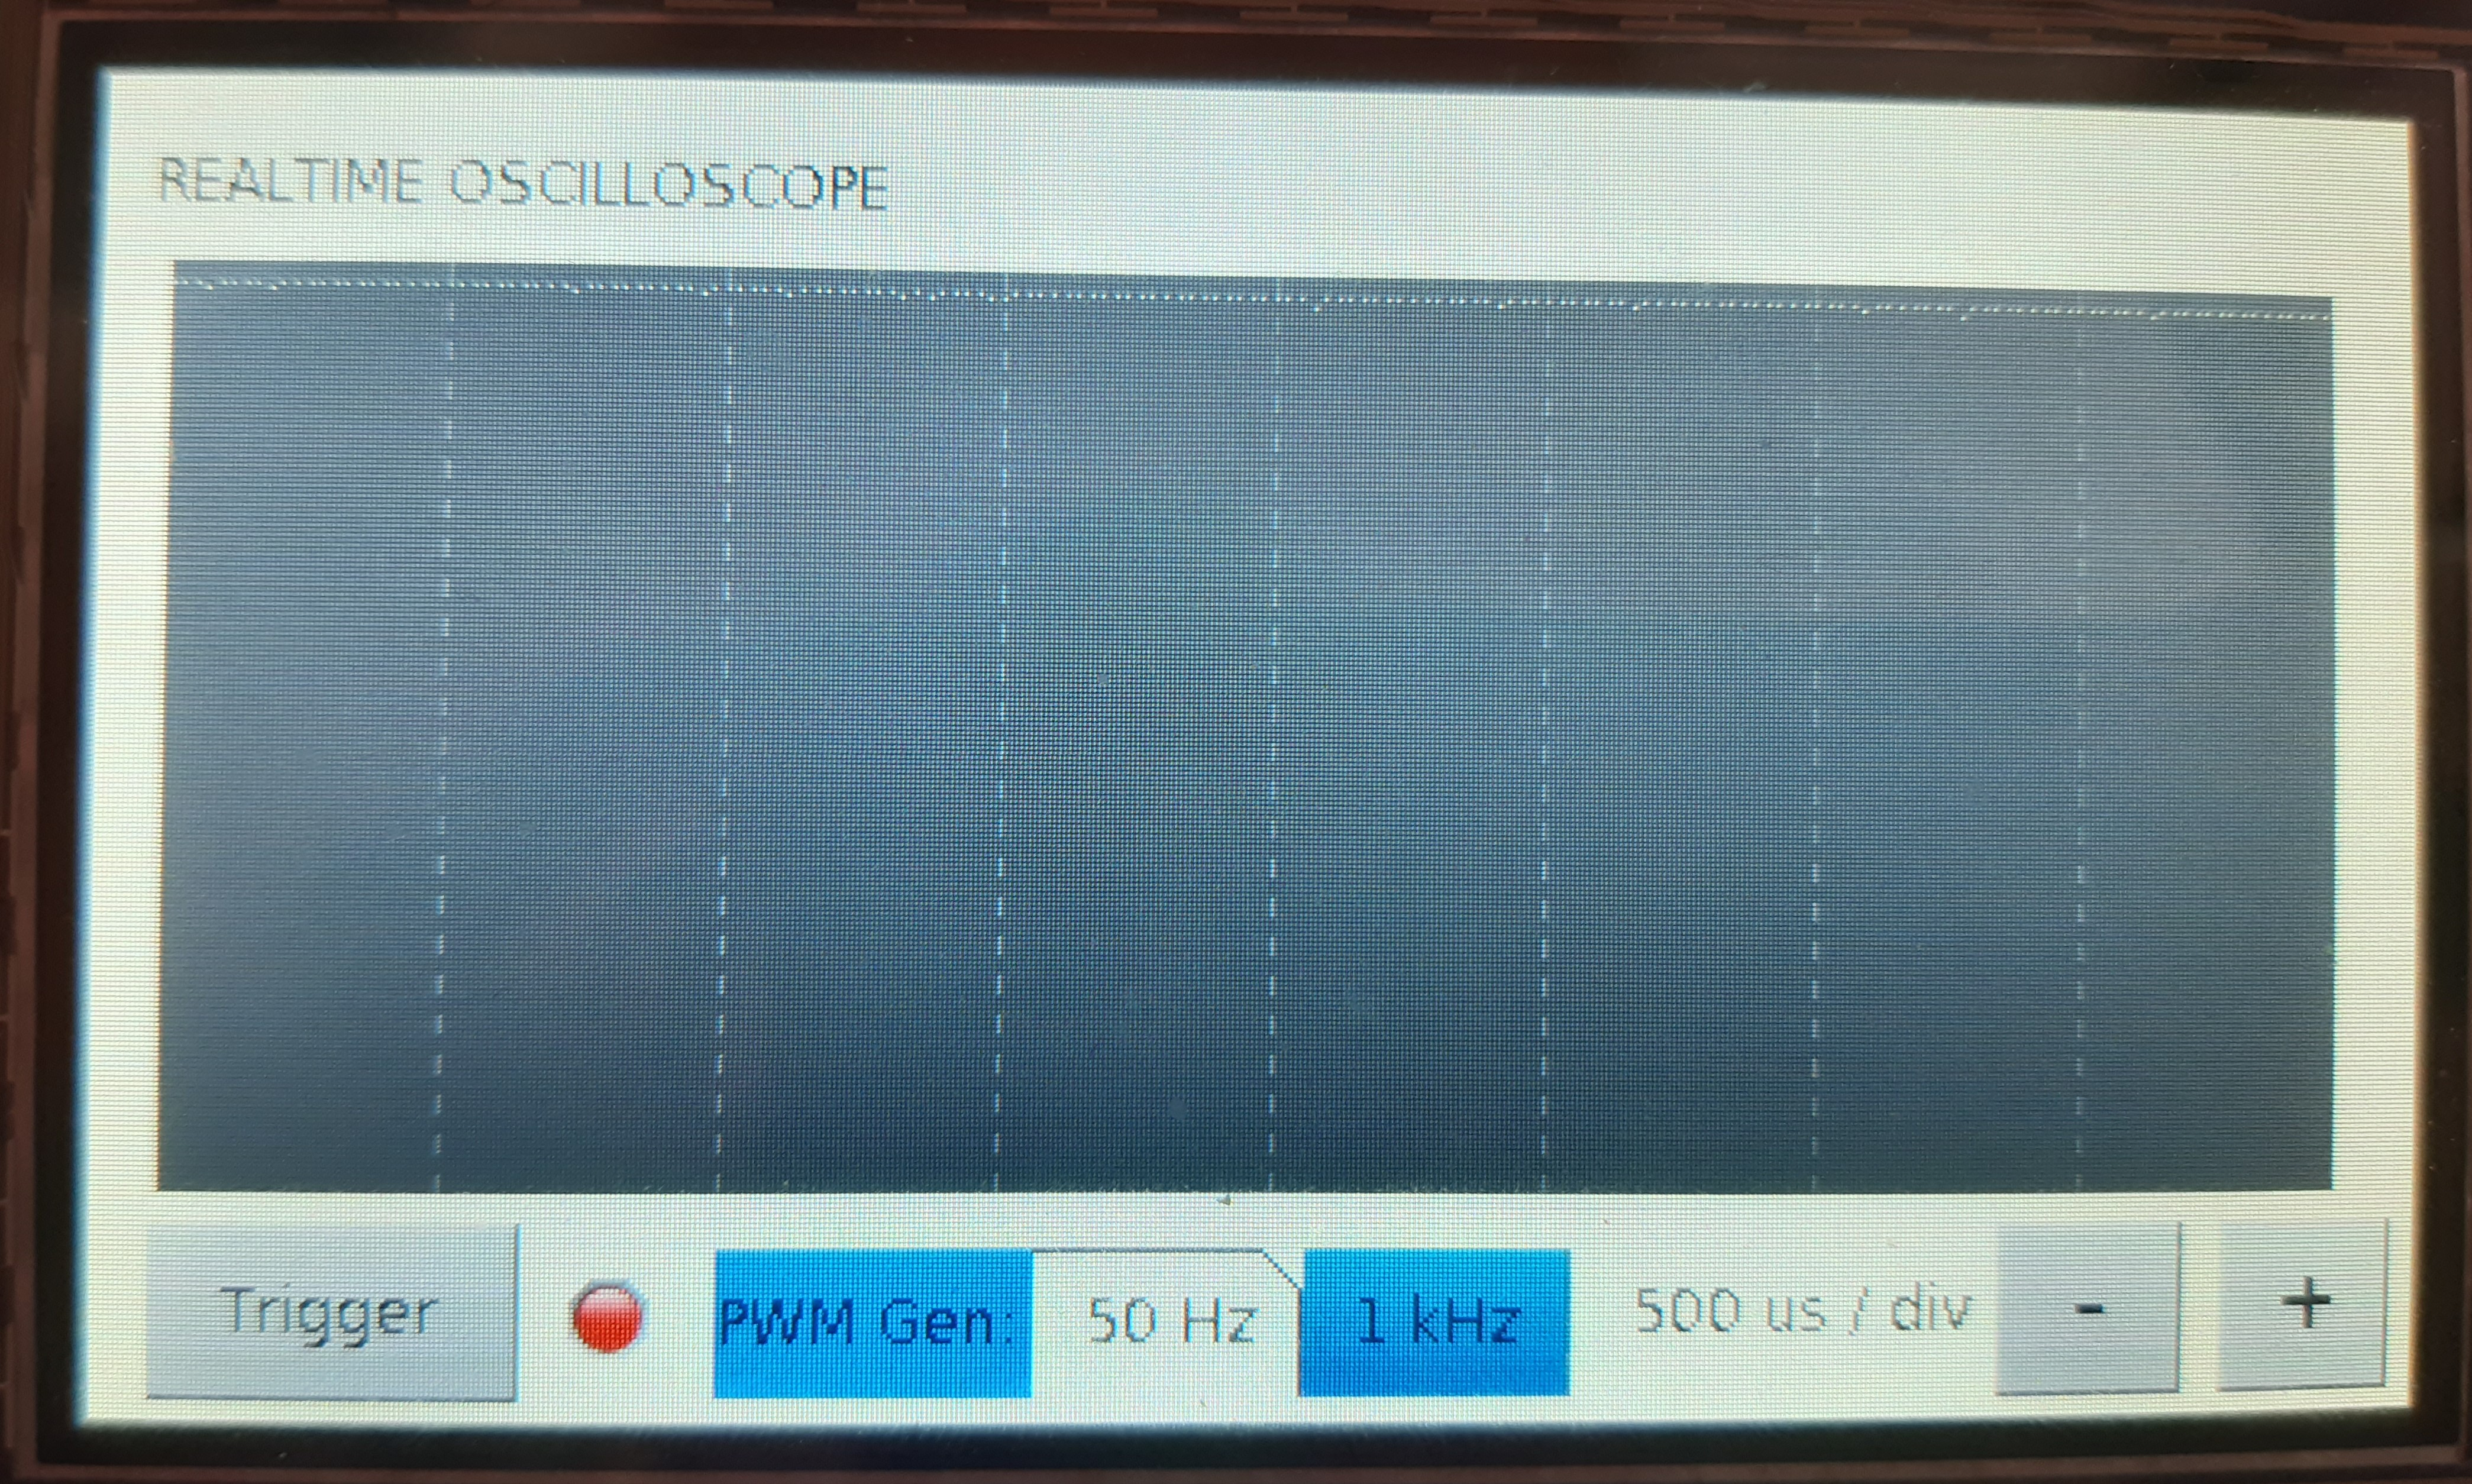
\includegraphics[scale=0.08]{Ressources/PWM_500us}\\ 
			\hline 
			\multicolumn{2}{|c|}{Final Conditions:}&\\ 
			\hline 
			\multicolumn{2}{|c|}{Comments:}&\\ 
			\hline 
			\multicolumn{2}{|c|}{Test Passed:}&Yes \\ 
			\hline 
		\end{tabular} 
	\end{center}
\end{table}	
		\begin{table}[H]
	\begin{center}
		\begin{tabular}{| m{2cm}|m{2cm}|m{12cm}|}
			\hline 
			\bf D2&\bf Title:&\bf Check if Sinus wave can be correclty visualised\\ 
			\hline 
			\multicolumn{2}{|c|}{Group:}&Signal Display\\ 
			\hline 
			\multicolumn{2}{|c|}{Description:}&50 Hz Signal with 10 ms/div time base\\ 
			\hline 
			\multicolumn{2}{|c|}{Initial Conditions:}&Sampling rate: 100kSamples/s\\ 
			\hline 
			\multicolumn{2}{|c|}{Test Results:}&The sampling frequency is high enough. There are enough points.
			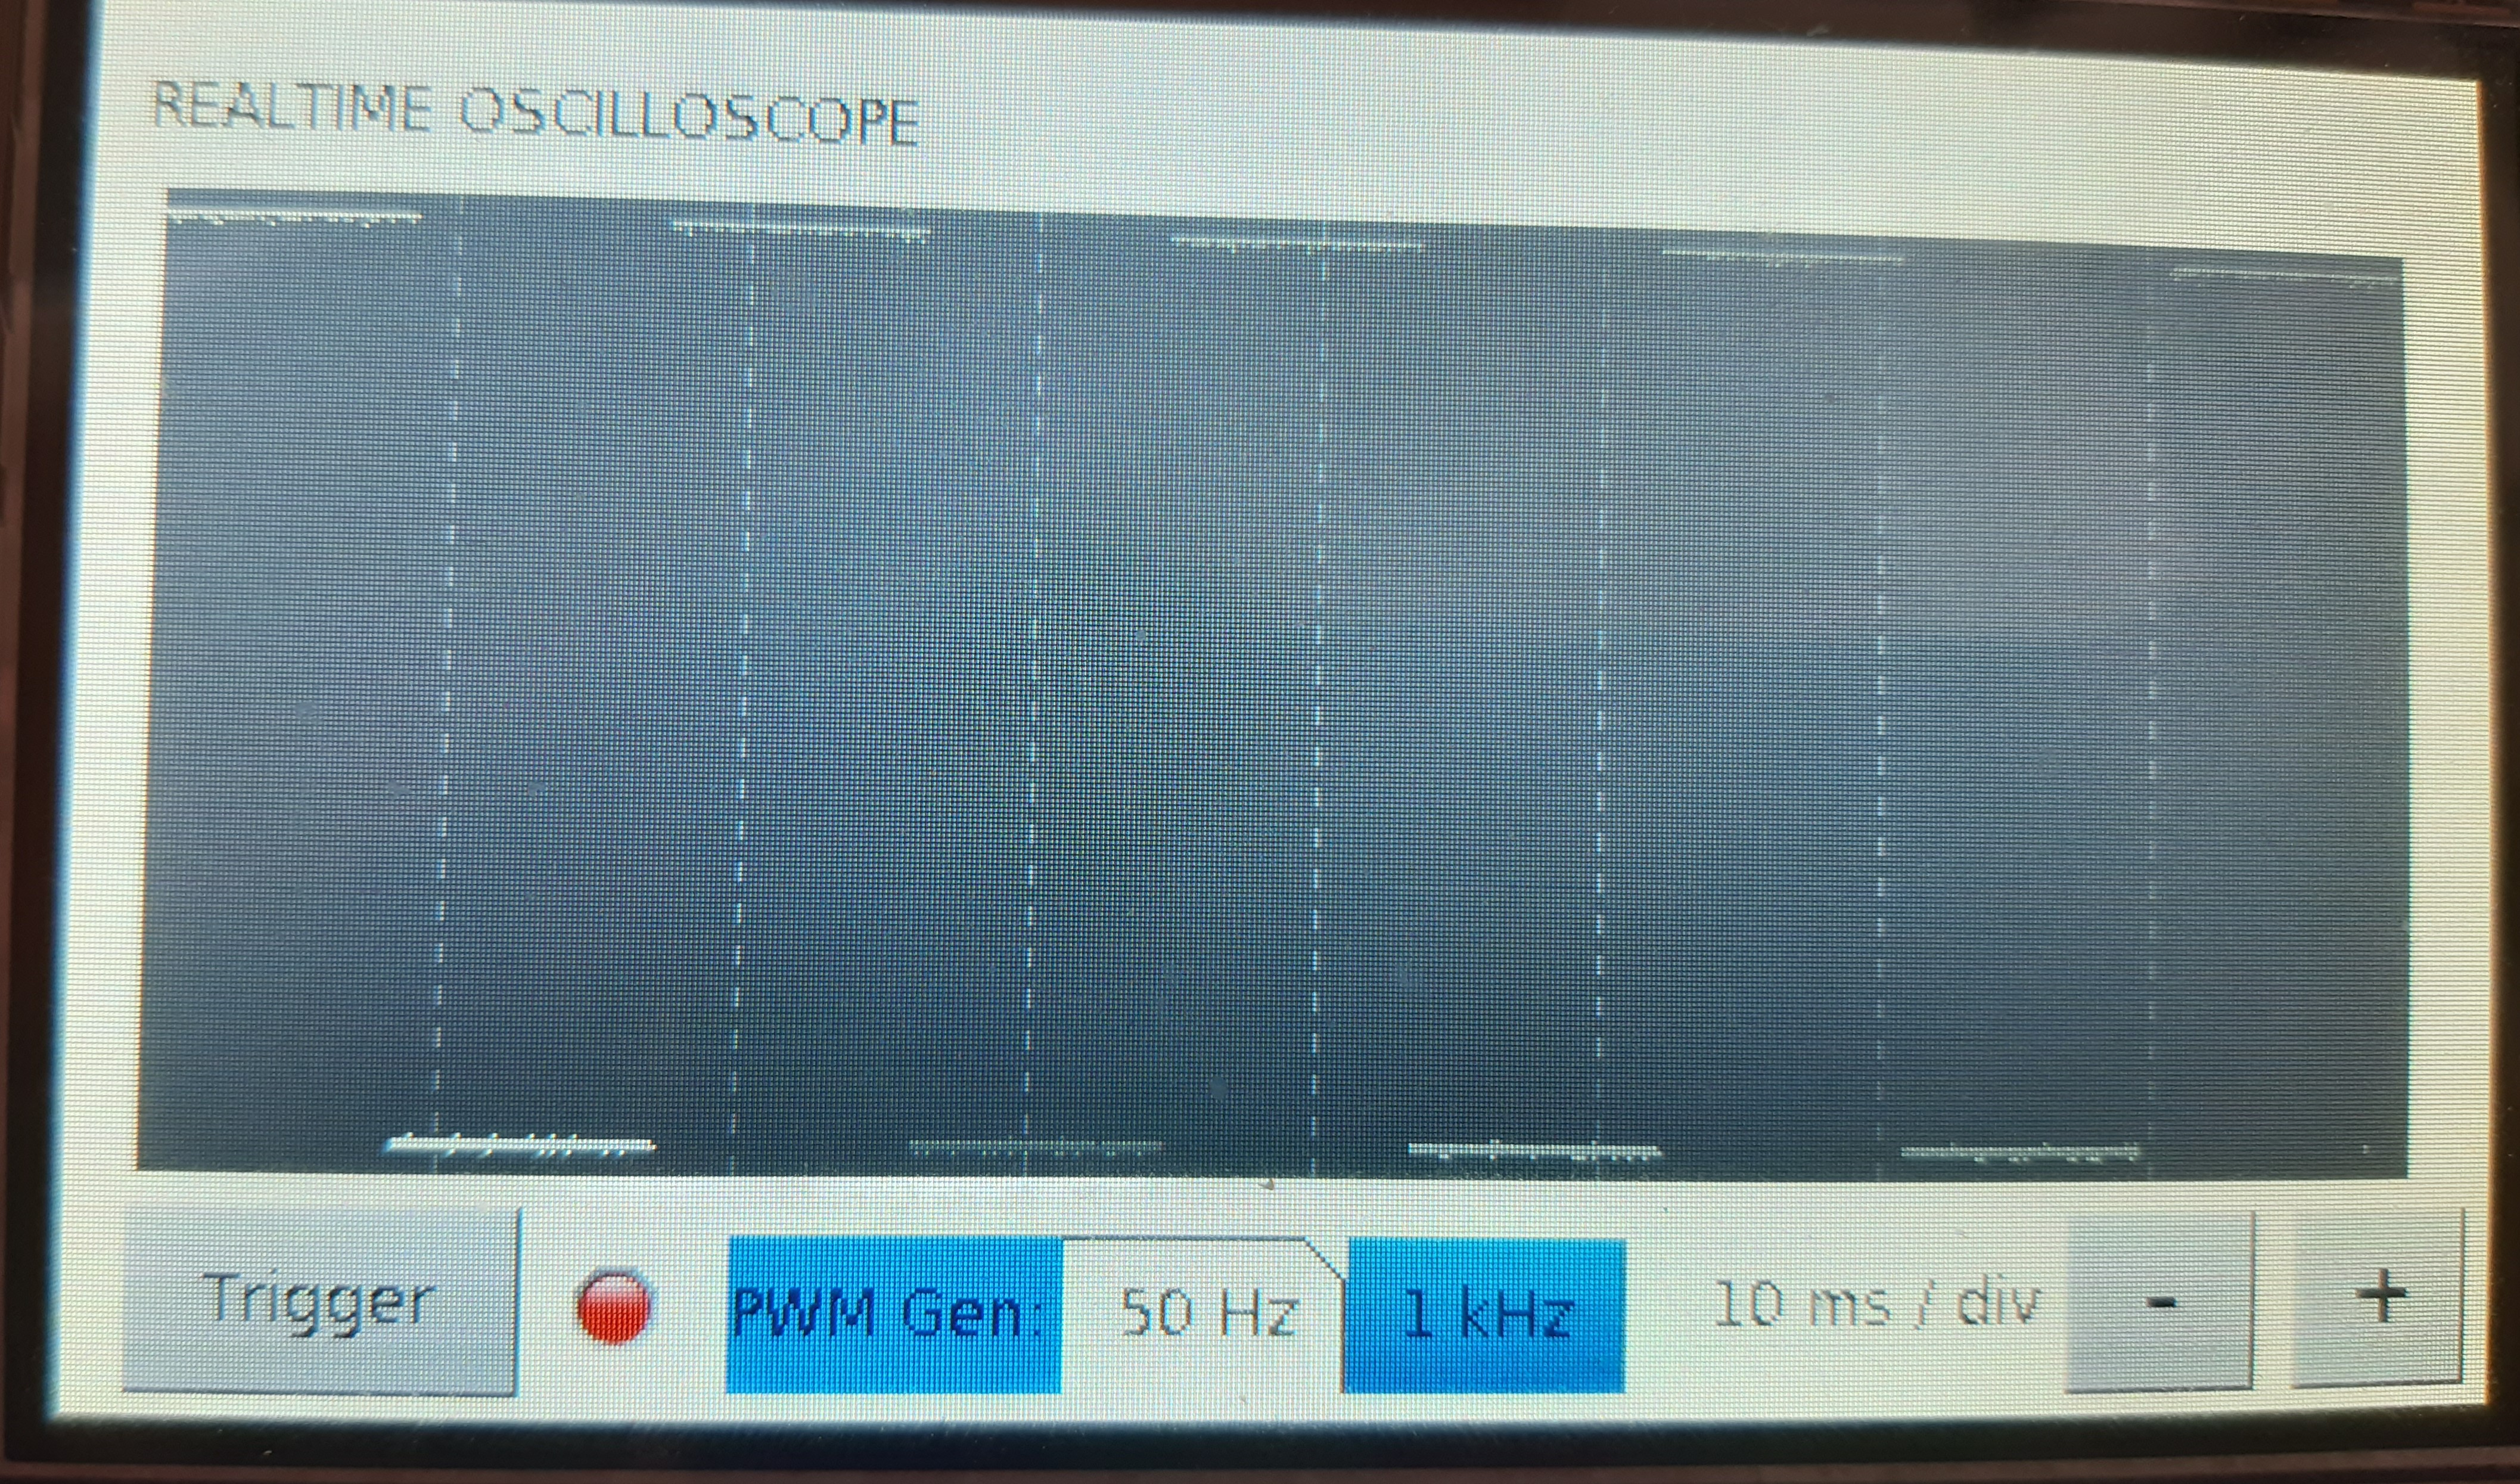
\includegraphics[scale=0.08]{Ressources/PWM_10ms}\\ 
			\hline 
			\multicolumn{2}{|c|}{Final Conditions:}&\\ 
			\hline 
			\multicolumn{2}{|c|}{Comments:}&\\ 
			\hline 
			\multicolumn{2}{|c|}{Test Passed:}&Yes \\ 
			\hline 
		\end{tabular} 
	\end{center}
\end{table}	
		\begin{table}[H]
	\begin{center}
		\begin{tabular}{| m{2cm}|m{2cm}|m{12cm}|}
			\hline 
			\bf D3&\bf Title:&\bf Check if Sinus wave can be correclty visualised\\ 
			\hline 
			\multicolumn{2}{|c|}{Group:}&Signal Display\\ 
			\hline 
			\multicolumn{2}{|c|}{Description:}&1 kHz Signal with 500 us/div time base\\ 
			\hline 
			\multicolumn{2}{|c|}{Initial Conditions:}&Sampling rate: 100kSamples/s\\ 
			\hline 
			\multicolumn{2}{|c|}{Test Results:}&The sampling frequency is high enough. There are enough points.
			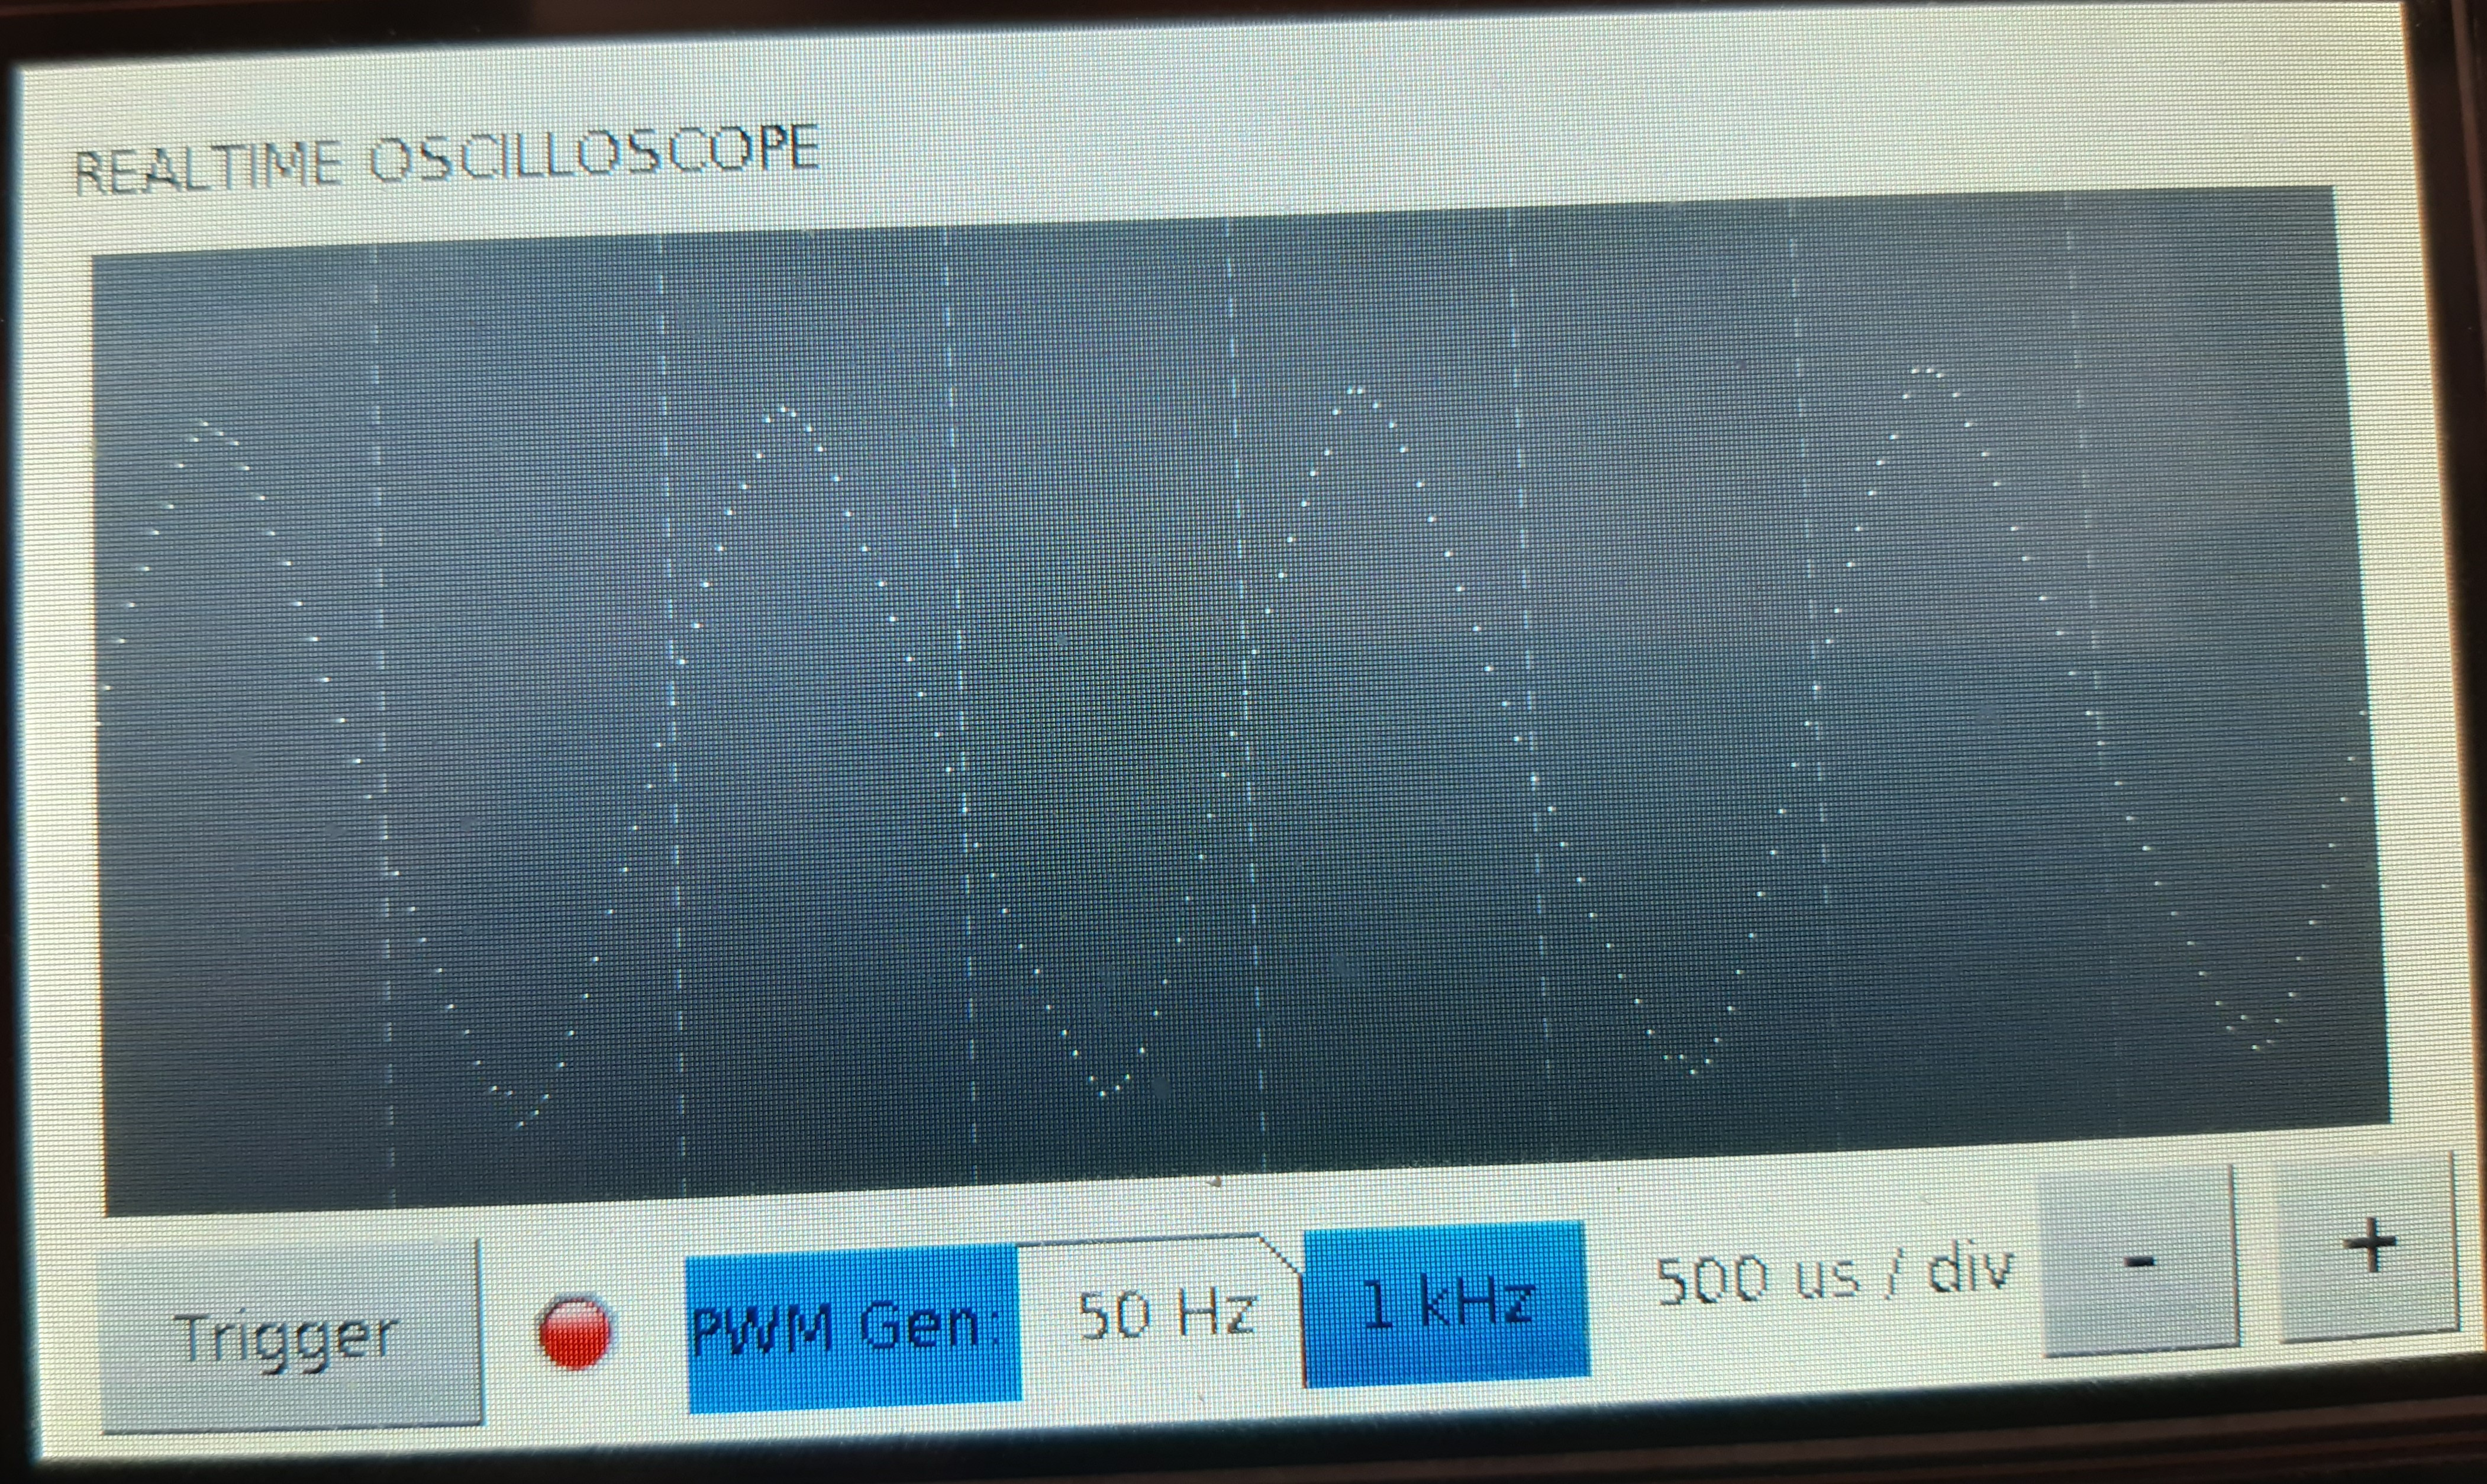
\includegraphics[scale=0.08]{Ressources/sinus_500us}\\ 
			\hline 
			\multicolumn{2}{|c|}{Final Conditions:}&\\ 
			\hline 
			\multicolumn{2}{|c|}{Comments:}&\\ 
			\hline 
			\multicolumn{2}{|c|}{Test Passed:}&Yes \\ 
			\hline 
		\end{tabular} 
	\end{center}
\end{table}	
		\begin{table}[H]
	\begin{center}
		\begin{tabular}{| m{2cm}|m{2cm}|m{12cm}|}
			\hline 
			\bf D4&\bf Title:&\bf Check if Sinus wave can be correclty visualised\\ 
			\hline 
			\multicolumn{2}{|c|}{Group:}&Signal Display\\ 
			\hline 
			\multicolumn{2}{|c|}{Description:}&1 kHz Signal with 10 ms/div time base\\ 
			\hline 
			\multicolumn{2}{|c|}{Initial Conditions:}&Sampling rate: 100kSamples/s\\ 
			\hline 
			\multicolumn{2}{|c|}{Test Results:}&The sampling frequency is high enough. There are enough points.
			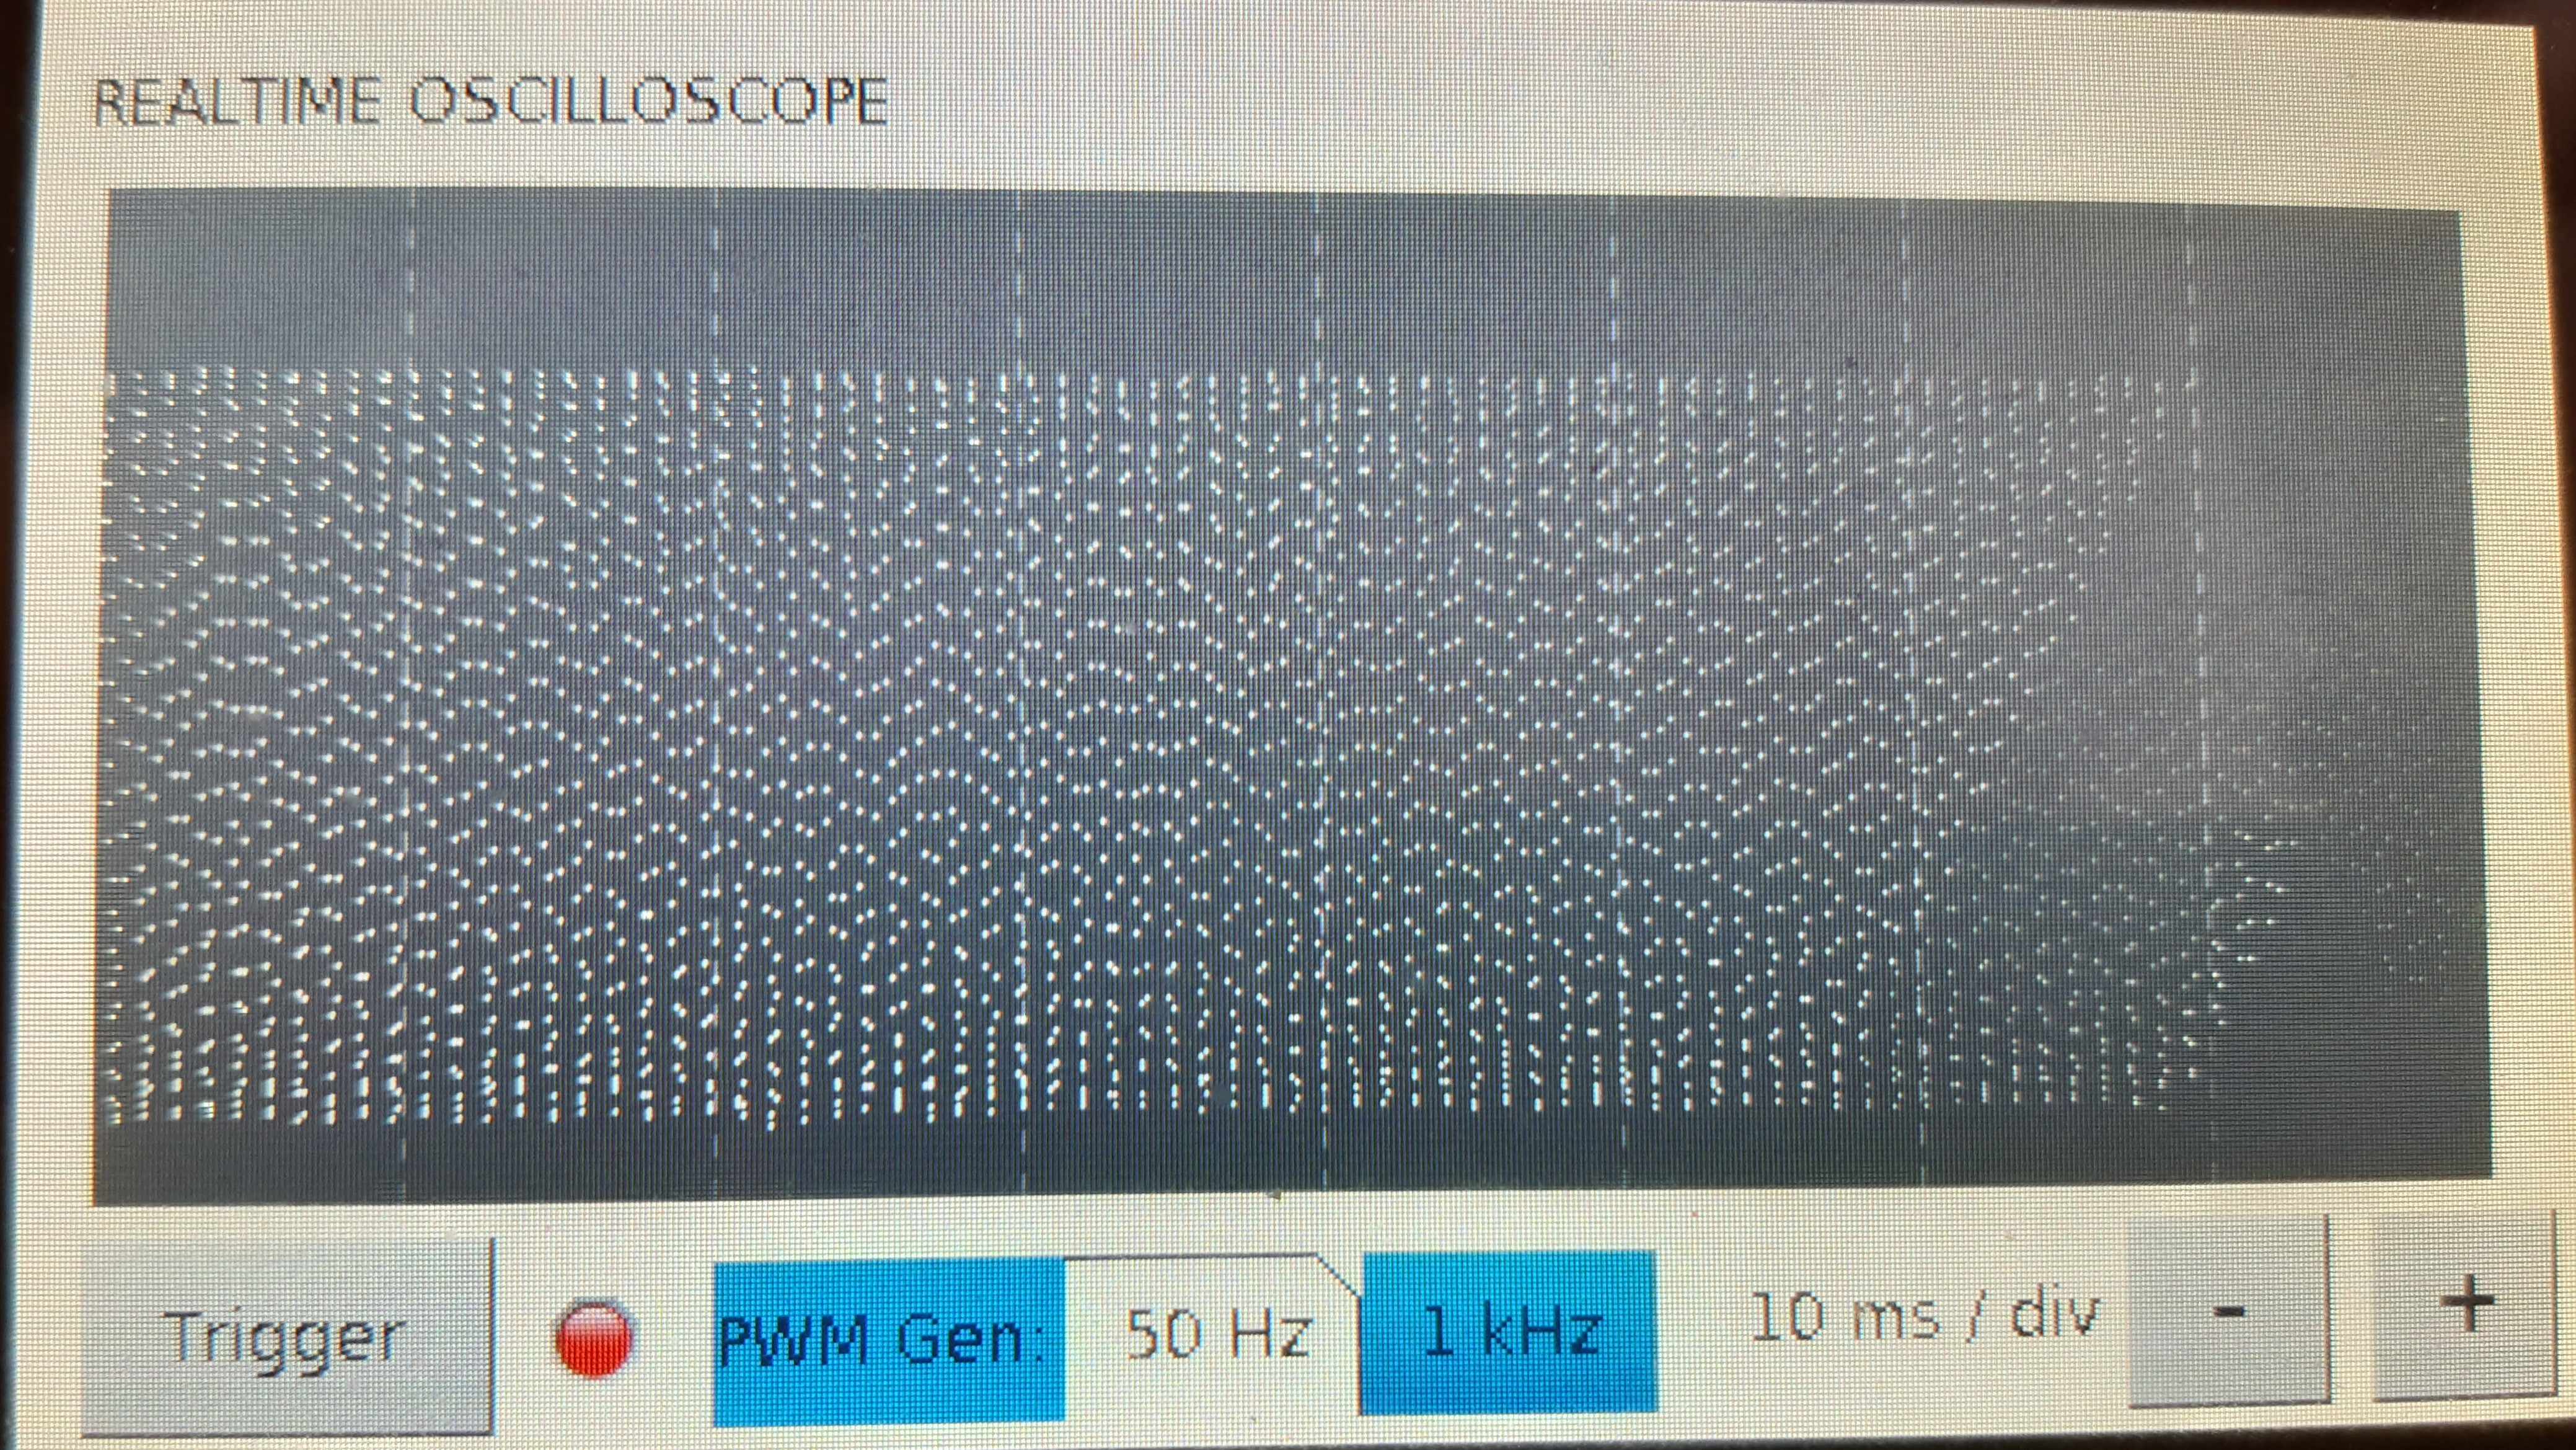
\includegraphics[scale=0.08]{Ressources/sinus_10ms}\\ 
			\hline 
			\multicolumn{2}{|c|}{Final Conditions:}&\\ 
			\hline 
			\multicolumn{2}{|c|}{Comments:}&\\ 
			\hline 
			\multicolumn{2}{|c|}{Test Passed:}&Yes \\ 
			\hline 
		\end{tabular} 
	\end{center}
\end{table}	
\subsection{E}
		\begin{table}[H]
	\begin{center}
		\begin{tabular}{| m{2cm}|m{2cm}|m{12cm}|}
			\hline 
			\bf E1&\bf Title:&\bf Check maximum display refresh rate\\ 
			\hline 
			\multicolumn{2}{|c|}{Group:}&Display Refresh Rate\\ 
			\hline 
			\multicolumn{2}{|c|}{Description:}&Display refresh rate: 50 Hz\\ 
			\hline 
			\multicolumn{2}{|c|}{Initial Conditions:}&Display refresh rate: 50 Hz\\ 
			\hline 
			\multicolumn{2}{|c|}{Test Results:}&The refresh is correctly done\\ 
			\hline 
			\multicolumn{2}{|c|}{Final Conditions:}&\\ 
			\hline 
			\multicolumn{2}{|c|}{Comments:}&\\ 
			\hline 
			\multicolumn{2}{|c|}{Test Passed:}&Yes \\ 
			\hline 
		\end{tabular} 
	\end{center}
\end{table}	
		\begin{table}[H]
	\begin{center}
		\begin{tabular}{| m{2cm}|m{2cm}|m{12cm}|}
			\hline 
			\bf E2&\bf Title:&\bf Check maximum display refresh rate\\ 
			\hline 
			\multicolumn{2}{|c|}{Group:}&Display Refresh Rate\\ 
			\hline 
			\multicolumn{2}{|c|}{Description:}&Display refresh rate: 66 Hz\\ 
			\hline 
			\multicolumn{2}{|c|}{Initial Conditions:}&Display refresh rate: 66 Hz\\ 
			\hline 
			\multicolumn{2}{|c|}{Test Results:}&The refresh is correctly done\\ 
			\hline 
			\multicolumn{2}{|c|}{Final Conditions:}&\\ 
			\hline 
			\multicolumn{2}{|c|}{Comments:}&\\ 
			\hline 
			\multicolumn{2}{|c|}{Test Passed:}&Yes \\ 
			\hline 
		\end{tabular} 
	\end{center}
\end{table}	
		\begin{table}[H]
	\begin{center}
		\begin{tabular}{| m{2cm}|m{2cm}|m{12cm}|}
			\hline 
			\bf E3&\bf Title:&\bf Check maximum display refresh rate\\ 
			\hline 
			\multicolumn{2}{|c|}{Group:}&Display Refresh Rate\\ 
			\hline 
			\multicolumn{2}{|c|}{Description:}&Display refresh rate: 100 Hz\\ 
			\hline 
			\multicolumn{2}{|c|}{Initial Conditions:}&Display refresh rate: 100 Hz\\ 
			\hline 
			\multicolumn{2}{|c|}{Test Results:}&The refresh is correctly done\\ 
			\hline 
			\multicolumn{2}{|c|}{Final Conditions:}&\\ 
			\hline 
			\multicolumn{2}{|c|}{Comments:}&There are no difference between all these tests. The measured duration of a refresh is 22 ms. 
			So the uC is refreshing all the time as fast as possible, even with the 50 Hz refresh rate.\\ 
			\hline 
			\multicolumn{2}{|c|}{Test Passed:}&Yes \\ 
			\hline 
		\end{tabular} 
	\end{center}
\end{table}	
\subsection{F}
		\begin{table}[H]%%
	\begin{center}
		\begin{tabular}{| m{2cm}|m{2cm}|m{12cm}|}
			\hline 
			\bf F1&\bf Title:&\bf Check if changes of x-axis scaling take effect on signal view\\ 
			\hline 
			\multicolumn{2}{|c|}{Group:}&Time Divisions Display\\ 
			\hline 
			\multicolumn{2}{|c|}{Description:}&From 500 us/div to 1 ms/div\\ 
			\hline 
			\multicolumn{2}{|c|}{Initial Conditions:}&Input signal: square 1kHz, Div: 500 us\\ 
			\hline 
			\multicolumn{2}{|c|}{Test Results:}&The signal changes accordingly\\ 
			\hline 
			\multicolumn{2}{|c|}{Final Conditions:}&Div: 1 ms\\ 
			\hline 
			\multicolumn{2}{|c|}{Comments:}&\\ 
			\hline 
			\multicolumn{2}{|c|}{Test Passed:}&Yes \\ 
			\hline 
		\end{tabular} 
	\end{center}
\end{table}	
		\begin{table}[H]
	\begin{center}
		\begin{tabular}{| m{2cm}|m{2cm}|m{12cm}|}
			\hline 
			\bf F2&\bf Title:&\bf Check if changes of x-axis scaling take effect on signal view\\ 
			\hline 
			\multicolumn{2}{|c|}{Group:}&Time Divisions Display\\ 
			\hline 
			\multicolumn{2}{|c|}{Description:}&From 1 ms/div to 2 ms/div\\ 
			\hline 
			\multicolumn{2}{|c|}{Initial Conditions:}&Input signal: square 1kHz, Div: 1 ms\\ 
			\hline 
			\multicolumn{2}{|c|}{Test Results:}&The signal changes accordingly\\ 
			\hline 
			\multicolumn{2}{|c|}{Final Conditions:}&Div: 2 ms \\ 
			\hline 
			\multicolumn{2}{|c|}{Comments:}&\\ 
			\hline 
			\multicolumn{2}{|c|}{Test Passed:}&Yes \\ 
			\hline 
		\end{tabular} 
	\end{center}
\end{table}	
		\begin{table}[H]
	\begin{center}
		\begin{tabular}{| m{2cm}|m{2cm}|m{12cm}|}
			\hline 
			\bf F3&\bf Title:&\bf Check if changes of x-axis scaling take effect on signal view\\ 
			\hline 
			\multicolumn{2}{|c|}{Group:}&Time Divisions Display\\ 
			\hline 
			\multicolumn{2}{|c|}{Description:}&From 2 ms/div to 5 ms/div\\ 
			\hline 
			\multicolumn{2}{|c|}{Initial Conditions:}&Input signal: square 1kHz, Div: 2 ms\\ 
			\hline 
			\multicolumn{2}{|c|}{Test Results:}&The signal changes accordingly\\ 
			\hline 
			\multicolumn{2}{|c|}{Final Conditions:}&Div: 5 ms\\ 
			\hline 
			\multicolumn{2}{|c|}{Comments:}&\\ 
			\hline 
			\multicolumn{2}{|c|}{Test Passed:}&Yes \\ 
			\hline 
		\end{tabular} 
	\end{center}
\end{table}	
		\begin{table}[H]
	\begin{center}
		\begin{tabular}{| m{2cm}|m{2cm}|m{12cm}|}
			\hline 
			\bf F4&\bf Title:&\bf Check if changes of x-axis scaling take effect on signal view\\ 
			\hline 
			\multicolumn{2}{|c|}{Group:}&Time Divisions Display\\ 
			\hline 
			\multicolumn{2}{|c|}{Description:}&From 5 ms/div to 10 ms/div\\ 
			\hline 
			\multicolumn{2}{|c|}{Initial Conditions:}&Input signal: square 50 Hz, Div: 5 ms\\ 
			\hline 
			\multicolumn{2}{|c|}{Test Results:}&The signal changes accordingly\\ 
			\hline 
			\multicolumn{2}{|c|}{Final Conditions:}&Div: 10 ms \\ 
			\hline 
			\multicolumn{2}{|c|}{Comments:}&\\ 
			\hline 
			\multicolumn{2}{|c|}{Test Passed:}&Yes \\ 
			\hline 
		\end{tabular} 
	\end{center}
\end{table}	
		\begin{table}[H]
	\begin{center}
		\begin{tabular}{| m{2cm}|m{2cm}|m{12cm}|}
			\hline 
			\bf F5&\bf Title:&\bf Check if changes of x-axis scaling take effect on signal view\\ 
			\hline 
			\multicolumn{2}{|c|}{Group:}&Time Divisions Display\\ 
			\hline 
			\multicolumn{2}{|c|}{Description:}&From 10 ms/div back to 5 ms/div\\ 
			\hline 
			\multicolumn{2}{|c|}{Initial Conditions:}&Input signal: square 50 Hz, Div: 10 ms\\ 
			\hline 
			\multicolumn{2}{|c|}{Test Results:}&The signal changes accordingly\\ 
			\hline 
			\multicolumn{2}{|c|}{Final Conditions:}&Div: 5 ms\\ 
			\hline 
			\multicolumn{2}{|c|}{Comments:}&\\ 
			\hline 
			\multicolumn{2}{|c|}{Test Passed:}&Yes \\ 
			\hline 
		\end{tabular} 
	\end{center}
\end{table}	
		\begin{table}[H]
	\begin{center}
		\begin{tabular}{| m{2cm}|m{2cm}|m{12cm}|}
			\hline 
			\bf F6&\bf Title:&\bf Check if changes of x-axis scaling take effect on signal view\\ 
			\hline 
			\multicolumn{2}{|c|}{Group:}&Time Divisions Display\\ 
			\hline 
			\multicolumn{2}{|c|}{Description:}&From 5 ms/div back to 2 ms/div\\ 
			\hline 
			\multicolumn{2}{|c|}{Initial Conditions:}&Input signal: square 50 Hz, Div: 5 ms\\ 
			\hline 
			\multicolumn{2}{|c|}{Test Results:}&The signal changes accordingly\\ 
			\hline 
			\multicolumn{2}{|c|}{Final Conditions:}&Div: 2 ms\\ 
			\hline 
			\multicolumn{2}{|c|}{Comments:}&\\ 
			\hline 
			\multicolumn{2}{|c|}{Test Passed:}&Yes \\ 
			\hline 
		\end{tabular} 
	\end{center}
\end{table}	
		\begin{table}[H]
	\begin{center}
		\begin{tabular}{| m{2cm}|m{2cm}|m{12cm}|}
			\hline 
			\bf F7&\bf Title:&\bf Check if changes of x-axis scaling take effect on signal view\\ 
			\hline 
			\multicolumn{2}{|c|}{Group:}&Time Divisions Display\\ 
			\hline 
			\multicolumn{2}{|c|}{Description:}&From 2 ms/div to 1 ms/div\\ 
			\hline 
			\multicolumn{2}{|c|}{Initial Conditions:}&Input signal: square 1kHz, Div: 2 ms\\ 
			\hline 
			\multicolumn{2}{|c|}{Test Results:}&The signal changes accordingly\\ 
			\hline 
			\multicolumn{2}{|c|}{Final Conditions:}&Div: 1 ms \\ 
			\hline 
			\multicolumn{2}{|c|}{Comments:}&\\ 
			\hline 
			\multicolumn{2}{|c|}{Test Passed:}&Yes \\ 
			\hline 
		\end{tabular} 
	\end{center}
\end{table}	
		\begin{table}[H]
	\begin{center}
		\begin{tabular}{| m{2cm}|m{2cm}|m{12cm}|}
			\hline 
			\bf F8&\bf Title:&\bf Check if changes of x-axis scaling take effect on signal view\\ 
			\hline 
			\multicolumn{2}{|c|}{Group:}&Time Divisions Display\\ 
			\hline 
			\multicolumn{2}{|c|}{Description:}&From 1 ms/div to 500 us/div\\ 
			\hline 
			\multicolumn{2}{|c|}{Initial Conditions:}&Input signal: square 1kHz, Div: 1 ms\\ 
			\hline 
			\multicolumn{2}{|c|}{Test Results:}&The signal changes accordingly\\ 
			\hline 
			\multicolumn{2}{|c|}{Final Conditions:}&Div: 500 us\\ 
			\hline 
			\multicolumn{2}{|c|}{Comments:}&\\ 
			\hline 
			\multicolumn{2}{|c|}{Test Passed:}&Yes \\ 
			\hline 
		\end{tabular} 
	\end{center}
\end{table}	
\subsection{G}
		\begin{table}[H]
	\begin{center}
		\begin{tabular}{| m{2cm}|m{2cm}|m{12cm}|}
			\hline 
			\bf G1-5&\bf Title:&\bf Check if when enabling signal triggering, the periodic signal stays still on the display\\ 
			\hline 
			\multicolumn{2}{|c|}{Group:}&Trigger Signal Display\\ 
			\hline 
			\multicolumn{2}{|c|}{Description:}&Enable the triggering, and change the time base\\ 
			\hline 
			\multicolumn{2}{|c|}{Initial Conditions:}&Input signal: 50Hz square, Div: 500us\\ 
			\hline 
			\multicolumn{2}{|c|}{Test Results:}&The periodic signal stay still on the display, but sometimes it moves just for 1 frame.\\ 
			\hline 
			\multicolumn{2}{|c|}{Final Conditions:}&Div: 10 ms\\ 
			\hline 
			\multicolumn{2}{|c|}{Comments:}&\\ 
			\hline 
			\multicolumn{2}{|c|}{Test Passed:}&Partially \\ 
			\hline 
		\end{tabular} 
	\end{center}
\end{table}	
		\begin{table}[H]
	\begin{center}
		\begin{tabular}{| m{2cm}|m{2cm}|m{12cm}|}
			\hline 
			\bf G6-10&\bf Title:&\bf Check if when enabling signal triggering, the periodic signal stays still on the display\\ 
			\hline 
			\multicolumn{2}{|c|}{Group:}&Trigger Signal Display\\ 
			\hline 
			\multicolumn{2}{|c|}{Description:}&Enable the triggering, and change the time base\\ 
			\hline 
			\multicolumn{2}{|c|}{Initial Conditions:}&Input signal: 1kHz triangle, Div: 500us\\ 
			\hline 
			\multicolumn{2}{|c|}{Test Results:}&The periodic signal stay still on the display, but sometimes it moves just for 1 frame.\\ 
			\hline 
			\multicolumn{2}{|c|}{Final Conditions:}&Div: 10 ms\\ 
			\hline 
			\multicolumn{2}{|c|}{Comments:}&\\ 
			\hline 
			\multicolumn{2}{|c|}{Test Passed:}&Partially \\ 
			\hline 
		\end{tabular} 
	\end{center}
\end{table}	
		\begin{table}[H]
	\begin{center}
		\begin{tabular}{| m{2cm}|m{2cm}|m{12cm}|}
			\hline 
			\bf G11-15&\bf Title:&\bf Check if when enabling signal triggering, the periodic signal stays still on the display\\ 
			\hline 
			\multicolumn{2}{|c|}{Group:}&Trigger Signal Display\\ 
			\hline 
			\multicolumn{2}{|c|}{Description:}&Enable the triggering, and change the time base\\ 
			\hline 
			\multicolumn{2}{|c|}{Initial Conditions:}&Input signal: 1kHz sinus, Div: 500us\\ 
			\hline 
			\multicolumn{2}{|c|}{Test Results:}&The periodic signal stay still on the display, but sometimes it moves just for 1 frame.\\ 
			\hline 
			\multicolumn{2}{|c|}{Final Conditions:}&Div: 10 ms\\ 
			\hline 
			\multicolumn{2}{|c|}{Comments:}&\\ 
			\hline 
			\multicolumn{2}{|c|}{Test Passed:}&Partially \\ 
			\hline 
		\end{tabular} 
	\end{center}
\end{table}	

\subsection{L}
		\begin{table}[H]
	\begin{center}
		\begin{tabular}{| m{2cm}|m{2cm}|m{12cm}|}
			\hline 
			\bf L1&\bf Title:&\bf Does the software hang after a while?\\ 
			\hline 
			\multicolumn{2}{|c|}{Group:}&Long-Term Test\\ 
			\hline 
			\multicolumn{2}{|c|}{Description:}&Check if the system is running without user interaction for about 5 minutes\\ 
			\hline 
			\multicolumn{2}{|c|}{Initial Conditions:}&With RTOS\\ 
			\hline 
			\multicolumn{2}{|c|}{Test Results:}&The system still run correctly\\ 
			\hline 
			\multicolumn{2}{|c|}{Final Conditions:}&\\ 
			\hline 
			\multicolumn{2}{|c|}{Comments:}&\\ 
			\hline 
			\multicolumn{2}{|c|}{Test Passed:}&Yes \\ 
			\hline 
		\end{tabular} 
	\end{center}
\end{table}	
		\begin{table}[H]
	\begin{center}
		\begin{tabular}{| m{2cm}|m{2cm}|m{12cm}|}
			\hline 
			\bf L2&\bf Title:&\bf Does the software hang after a while?\\ 
			\hline 
			\multicolumn{2}{|c|}{Group:}&Long-Term Test\\ 
			\hline 
			\multicolumn{2}{|c|}{Description:}&Check if system is running with continuous user interaction for about 5 minutes\\ 
			\hline 
			\multicolumn{2}{|c|}{Initial Conditions:}&With RTOS\\ 
			\hline 
			\multicolumn{2}{|c|}{Test Results:}&The system still run correctly\\ 
			\hline 
			\multicolumn{2}{|c|}{Final Conditions:}&\\ 
			\hline 
			\multicolumn{2}{|c|}{Comments:}&\\ 
			\hline 
			\multicolumn{2}{|c|}{Test Passed:}&Yes \\ 
			\hline 
		\end{tabular} 
	\end{center}
\end{table}	
		\begin{table}[H]
	\begin{center}
		\begin{tabular}{| m{2cm}|m{2cm}|m{12cm}|}
			\hline 
			\bf L3&\bf Title:&\bf Does the software hang after a while?\\
			\hline 
			\multicolumn{2}{|c|}{Group:}&Long-Term Test\\ 
			\hline 
			\multicolumn{2}{|c|}{Description:}&Check if system is running for more then 6 hours\\ 
			\hline 
			\multicolumn{2}{|c|}{Initial Conditions:}&With RTOS\\ 
			\hline 
			\multicolumn{2}{|c|}{Test Results:}&The system still run correctly\\ 
			\hline 
			\multicolumn{2}{|c|}{Final Conditions:}&\\ 
			\hline 
			\multicolumn{2}{|c|}{Comments:}&\\ 
			\hline 
			\multicolumn{2}{|c|}{Test Passed:}&Yes \\ 
			\hline 
		\end{tabular} 
	\end{center}
\end{table}	

\subsection{Summary}

			\begin{table}[H]
		\begin{center}
			\begin{tabular}{| m{6cm}|m{2cm}|}
				\hline 
				\bf Total Tests:&\bf 31\\
				\hline 
				Tests passed:&27\\ 
				\hline 
				Tests partially passed:&3\\ 
				\hline 
				Tests not passed:&1\\ 
				\hline 
			\end{tabular} 
		\end{center}
	\end{table}	

	\section{Conclusion}
	Le but de ce projet était de réaliser un oscilloscope en temps réel. On peut dire que l'objectif est atteint car la majorité des tests ont été passés. Ce labo m'a permis de mieux comprendre les notions de temps réel abordées en cours, et de mieux maîtriser des outils tel que cubeMX ou encore System Workbench for STM32.
\end{document}
